\documentclass[conference,compsoc,a4paper,twocolumn,final]{IEEEtran}

%%{{{ Packages

\usepackage[utf8]{inputenc}
\usepackage[T1]{fontenc}
\usepackage{lmodern}
\usepackage{couriers}

\ifCLASSOPTIONcompsoc
  % IEEE Computer Society needs nocompress option
  % requires cite.sty v4.0 or later (November 2003)
  \usepackage[nocompress]{cite}
\else
  % normal IEEE
  \usepackage{cite}
\fi

\ifCLASSINFOpdf
  \usepackage[pdftex]{graphicx}
  % declare the path(s) where your graphic files are
  \graphicspath{../images/}
  % and their extensions so you won't have to specify these with
  % every instance of \includegraphics
  \DeclareGraphicsExtensions{.jpg,.png}
\else
  % or other class option (dvipsone, dvipdf, if not using dvips). graphicx
  % will default to the driver specified in the system graphics.cfg if no
  % driver is specified.
  % \usepackage[dvips]{graphicx}
  % declare the path(s) where your graphic files are
  % \graphicspath{{../eps/}}
  % and their extensions so you won't have to specify these with
  % every instance of \includegraphics
  % \DeclareGraphicsExtensions{.eps}
\fi

%% Package for non-breaking URL.
\usepackage{url}

%% \multirow{package}{width}{text}
\usepackage{multirow}

%% Package for reading CSV to database.
\usepackage{datatool}

%% Tikz
\usepackage{tikz}
\usetikzlibrary{backgrounds, shapes.geometric, positioning, patterns}

%% Pgfplots
\usepackage{pgfplots}

%% MnSymbol
\usepackage{MnSymbol}

%%}}}

%% Set spacing on table.
\renewcommand{\arraystretch}{1.5}
\setlength{\tabcolsep}{3pt}

%%% uncomment this to show overrule in black box
\overfullrule=2cm

\hyphenation{
	Be-ri-kut
	Ja-nu-a-ri
	SIGKDD
	Wiki-pedia
	a-kan
	a-ku-ra-si
	ang-ka
	ba-gai-ma-na
	bayes-ian
	ber-gu-na
	ber-kas
	ber-ma-sa-lah
	ber-mak-na
	bi-a-ya
	da-lam
	data-set
	de-ngan
	di-ha-sil-kan
	di-pi-lih
	di-sing-kat
	di-tam-bah-kan
	dis-krit
	fung-si
	ga-bung-an
	ke-las
	ke-le-mah-an
	ke-mung-ki-nan
	ke-tak-se-imbang-an
	lan-guage
	ma-yo-ri-tas
	me-laku-kan
	me-me-rik-sa
	me-mi-lih
	me-ne-rap-kan
	meng-a-pli-ka-si-kan
	meng-ge-ne-ra-li-sa-si
	me-ning-kat-kan
	me-nye-dia-kan
	me-nye-im-bang-kan
	me-sin
	me-thod
	me-to-de
	mem-vi-sua-li-sa-si
	meng-gu-na-kan
	meng-hi-lang-kan
	meng-hu-bung-kan
	meng-i-kut-kan
	meng-i-kuti
	meng-im-ple-men-ta-si-kan
	meng-in-di-ka-si-kan
	mi-sal-nya
	mung-kin
	o-ver-sam-pling
	pa-ra-lel
	pe-la-ti-han
	pe-mi-sah
	pe-nan-da
	pe-ne-li-ti-an
	pe-nu-li-san
	pe-nyun-ting
	pem-ban-ding
	pen-de-kat-an
	peng-kla-si-fi-ka-si
	peng-a-pli-ka-si-an
	per-for-man-si-nya
	po-ten-si-al
	pro-ba-bi-li-tas
	pro-ses
	sam-pel
	se-im-bang
	se-jum-lah
	sun-ting-an
	ting-kat
	un-der-sam-pling
	wa-lau-pun
}


\begin{document}

%%{{{ TITLE AND AUTHOR

\title{Detecting Vandalism on English Wikipedia using Cascaded Random Forest}

\author{%
	\IEEEauthorblockN{Dwi Hendratmo Widyantoro}
	\IEEEauthorblockA{%
		Sekolah Teknik Elektro dan Informatika\\
		Institut Teknologi Bandung\\
		Jl. Ganesha No 10, Bandung, Indonesia 40132\\
		Email: dwi@stei.itb.ac.id
	}
	\and
	\IEEEauthorblockN{Muhamad Sulhan}
	\IEEEauthorblockA{%
		Sekolah Teknik Elektro dan Informatika\\
		Institut Teknologi Bandung\\
		Jl. Ganesha No 10, Bandung, Indonesia 40132\\
		Email: ms@students.itb.ac.id
	}
}

\maketitle

%%}}}

%%{{{ ABSTRACT

\begin{abstract}
Wikipedia.org is an online encyclopedia which can edited by anyone.
Those feature has benefit, which make the article in Wikipedia rapidly
increased in size and can be fixed subsequently, and their drawbacks was prone
to vandalism in the forms of invalid information, deletion, ads, or meaningless
content.
This paper propose a framework for detecting vandalism on English Wikipedia
using machine learning technique by training Cascaded Random Forest (CRF)
classifier on English Wikipedia dataset (PAN-WVC-10) that has been resampled
using Local Neighbourhood SMOTE (LNSMOTE).
Those two methods then compared with Random Forest (RF) for classifier and
SMOTE for resampling.
The result of classifiers that has been tested on PAN-WVC-11 English dataset
showed that dataset resampled using LNSMOTE increase the true-positive rate
better than SMOTE in both classifiers, RF and CRF.
CRF using SMOTE with 200 stages and 1 tree gave the better result among others
with TPR value 0.9904.
From training computation time, CRF 1.6 times faster than RF in resampled
dataset.
\end{abstract}

%%}}}

%%{{{ INTRODUCTION

\section{Introduction}
\label{section:introduction}

Vandalism, according to Merriam-Webster's dictionary is willful or malicious
destruction or defacement of public or private property.
In the context of Wikipedia, vandalism can be in the form of malicious edit
which intention to give wrong information, or hiding information by deleting
the content, abusive content, ads, and/or meaningless text.
Finding and fixing the article that has been vandalized can disrupt the editor
from writing or expanding new article or others important tasks, and for the
reader they will get the wrong information or no information at all, due to
deletion.

Corpus that commonly used for learning vandalism on Wikipedia is PAN Wikipedia
Vandalism Corpus 2010 (PAN-WVC-10)
\cite{potthast:2010b}
or PAN Wikipedia Vandalism Corpus 2011 (PAN-WVC-11)
\cite{potthast:2010b}.
Both of the corpus have class imbalance problem.
PAN-WVC-10 for an English articles have 32,439 sample with only $2,394$ (7\%)
of them is vandalism, whereas PAN-WVC-11 for an English articles have $9,985$
sampel with only $1,144$ (8\%) of them are vandalism.

Training a classifier on imbalance dataset could lead to low performance.
This can be caused either by the minority class has low contribution to error
rate, which make the classifier bias to majority class, or some classifier
assume that class distribution is balanced, while in real world cases this
rarely happened.

RF has the disadvantage in their the computation time especially when training
the classification model.
For a large dataset with more than 10,000 samples (like the PAN-WVC-10 cases)
this could lead to hours of training time.
One of the solution is by using Cascaded Random Forest (CRF) framework proposed
by Bauman et al.
\cite{baumann2013cascaded}.
Their paper state that CRF give a fast training model time and increased
performance compared to RF.

This paper try to overcome the dataset imbalance problem on PAN-WVC-10 by
applying resample and classifier technique that has never been used before on
the dataset.
The PAN-WVC-10 dataset is resampled using Local Neighborhood SMOTE (LNSMOTE)
technique,
which proposed by Maciejewski and Stefanowski
\cite{maciejewski2011local}.
The result from resampling then trained using CRF classifier and compared with
RF classifier to see their performance.

This paper is organized as follow.
Section \ref{section:literature_study} briefly review the past works that has
been done on vandalism detection on Wikipedia, SMOTE, LNSMOTE, RF and CRF.
Section \ref{section:research_methodology} describe how the feature generated
from raw dataset and resampled before it was trained and tested on classifiers.
Section \ref{section:result_and_analysis} show the result from each classifier
on each dataset and their analysis.
Section \ref{section:conclusion} conclude the experiment and
give some possible future works that can be extended from this paper.

%%}}}

\section{Literature Study}
\label{section:literature_study}

This section review the previous work and techniques used for implementation in
this paper.

%%{{{ PREVIOUS WORKS
\subsection{Previous Workds}

Since 2008, vandalism detection in Wikipedia based on machine learning approach
became an interesting research topic.
Potthast \cite{potthast2008automatic} contribution is the first vandalism
detection approach using machine learning with textual and basic
metadata features using Logistic Regression classifier.
Smets \cite{smets08automaticvandalism} use Naive Bayes classifier on selected
words that representing vandalism edit and the first who use compression model
to detect vandalism in Wikipedia.
Itakura and Clarke \cite{itakura2009using} use Dynamic Markov Compression to
detect vandalism edit in Wikipedia.
Mola Velasco \cite{mola2012wikipedia} extend the Potthast research by adding
more textual features and word-list features.
Velasco win the \textit{1st International Competition on Wikipedia Vandalism
Detection}.
West et al. \cite{west2011multilingual} use spatial and temporal metadata
without required to check the text in article and revision.
Adler et al. \cite{adler2011wikipedia} build a vandalism detection system using
reputation called WikiTrust.
Adler et al. \cite{adler2011wikipedia} then combine their previous work with
natural language, spatial and temporal features.
West and Lee \cite{west2011multilingual} is the first who introduce
\textit{ex post facto} data as feature, where their prediction take the next
revision into consideration.
Vandalism detection system from West and Lee win the \textit{2nd International
Competition on Wikipedia Vandalism Detection}.
Harpalani et al. \cite{harpalani2011language} propose that vandalism has
a uniq and equal lingustic property, they then build a system for detecting
vandalism based on \textit{stylometric} analysis from vandalism edit with
\textit{context-free grammar} probabilistic model.
Their approach overcome feature based system with short pattern, which equalize
syntactic structure with token of text.
Following the trend of classifying on cross-language vandalism, Tran and
Christen \cite{tran2013cross} evaluated several classifier based on
language feature collected from number of article viewed every hours and the
history of their edit in Wikipedia.

Gotze \cite{gotze2014advanced} combine feature from
Adler et al. \cite{adler2011wikipedia},
Javanmardi et al. \cite{javanmardi2011vandalism},
Mola Velasco \cite{mola2012wikipedia},
Potthast et al. \cite{potthast2008automatic},
Wang and McKeown \cite{wang2010got}, and
West and Lee \cite{west2011multilingual}
with four additional and modified features.

To overcome imbalance problem, Gotze use the random oversampling technique
called
\textit{Synthetic Minority Over-sampling TEchnique} (SMOTE)
proposed by Chawla
\cite{chawla2002smote}.
Original and resampled dataset of PAN-WVC-10 then tested with two-class
classifier:
\textit{Logistic Regression},
\textit{RealAdaBoost},
\textit{Random Forest} (RF), dan
\textit{Bayesian Network}.
His evaluation on original dataset showed that RF give better result than
others classifiers.
The result from resampling dataset showed increasing in performance on all
classifiers except RF.

From the previous research, seven of them use PAN-WVC-10
\cite{adler2010detecting}
\cite{adler2011wikipedia}
\cite{gotze2014advanced}
\cite{harpalani2011language}
\cite{mola2012wikipedia}
\cite{wang2010got}
\cite{west2011multilingual},
with the best precision value is $0.86$, recall value $0.57$, and PR-AUC
$0.66$, which obtained by Velasco using Random Forest without resampling on
dataset.
Only two research that use PAN-WVC-11
\cite{gotze2014advanced}
\cite{west2011multilingual}
with the best result obtained by Gotze, $0.92$ on precision, $0.39$
on recall, and $0.74$ on PR-AUC.
%%}}}

%%{{{ SMOTE
\subsection{SMOTE}
\label{subsection:smote}

SMOTE (Synthetic Minority Over-sampling Technique) method, proposed by Chawla
\cite{chawla2002smote},
use oversampling approach in which the minority class are resampled by creating
their synthetic samples not by replacing majority sample with minority class.
Synthetic sample created by application, operated on feature space.

Synthetic sample created with the following procedure,
\begin{itemize}
\item Pick $k$ nearest neigbour of minority sample randomly.
\item Calculate the difference between feature vector sample with their
neighbours.
\item Multiply the differece with random real number, ranged between 0 to 1.
\item Add their result to new feature vector.
\end{itemize}

The synthetic sample will be created in random line segment between two
selected features.
This approach effectively stimulate the learning region from minority class
become larger without causing over-fitting.
%%}}}

%%{{{ LNSMOTE
\subsection{LNSMOTE}
\label{subsection:lnsmote}

SMOTE method has several weakness.
First, all sample for minority class is used, this could be a problem because
not all the samples have equal benefit for learning.
Minority sample in the boundary region between minority and majority class
usually result in misclassified rather than sample located in the center of
region.
Sample that located in the center may give a little contribution to classifier.
One of the method to overcome this problem is by using sample in boundary of
minority class instead in the center which proposed by Han et al.
\cite{han2005borderline}, called Borderline SMOTE.

Another weakness of SMOTE method is overgeneralization, where their method does
not take into consideration the distribution of minority sample in majority
class, or the outliers.
Maciejewski et al. introduced an extension of SMOTE called Local Neighbourhood
SMOTE (LNSMOTE) \cite{maciejewski2011local}
using modified version of Safe-Level SMOTE (SLSMOTE)
\cite{bunkhumpornpat2009safe}.
In SLSMOTE majority samples is take into consideration before creating
synthetic sample by calculating a coefficient called safe-level.
For each minority sample, count the number of their K-nearest-neighbours (KNN).
If KNN value is close to 0, then the sample will be considered as noise.
If KNN value is close ot $k$, then the sample can be said in safe region in
minority class.
The main idea was to create synthetic sample that close to safe region.

The SLSMOTE strategy has a problem especially when class distribution is bias
in which the minority class spread into small sub-region with low number
cardinality.
In this situation, creating synthetic sample with SLMOTE will cause an overlap
between class.
This problem is due to SLSMOTE find only KNN for minority class.
If the sample candidate does not located in region with densed minority class,
then some of their neighbours could be far from sample candidate or surrounded
by majority class samples.
LNSMOTE overcome this overlap problem by taking into consideration the local
neighbourhood of minority sample candidate that can provide the number of of
majority class around each of them.
%%}}}

%%{{{ RANDOM FOREST
\subsection{Random Forest}
\label{subsection:rf}

\textit{Random Forest} (RF)
is a combination of several decision tree such that each tree depends on the
value of random vector sampled independently and with equal distribution for
all trees in the forest
\cite{breiman2001random}.

There are three common paremeter in building RF.
The first parameter is the number of tree in forest ($n$),
the other two parameters are percentage of samples ($b$) and number of random
features ($m$) for building the tree.
All of the parameters are set before building each tree and their value is
constant.

Percentage of sample for training that was selected randomly usually two third
from overall samples, which left one third of them as out of bag (OOB) samples.
For number of random feature $m$, the common value is the root or log of all
features \cite{breiman2001random}.

Procedure to build RF is as follows.
Let $S$ be a training set.
After their parameter has been set, when building each tree, take $b$ samples
randomly from $S$ without replacement (sample that get selected can be picked
again in the next iteration).
This process also know as bootstrapping.
Samples that does not included in $b$ is called out-of-bag (OOB), which can be
used to calculate the misclassification rate.
From $b$ samples, take $m$ random features, and then build the tree using $b$
samples with $m$ number of features without pruning.
Repeat the process until the $n$-tree has been built.

Classification process on RF proceed as follows.
Given test set $T$, with the same number of features with $S$.
For each sample $t$ in $T$, insert the sample $t$ into each tree and collect
their classification result.
After $n$ tree or $n$ number of class, compute the majority class from all
tree classification.
%%}}}

%%{{{ CASCADED RANDOM FOREST
\subsection{Cascaded Random Forest}
\label{subsection:crf}

A common problem in data mining or in ensemble learning algorithm is their
incapability on handling imbalance training data.
Inequality between positive and negative class usually result in low
detection accuracy.
A simulation run by Strobel et al. \cite{strobl2007bias} showed that RF skewed
in favor of majority class.
When using RF for detection, a vast amount of negative samples is required to
get a robust classifier with low false-positive rate, but this also cause an
inequality between positive and negative samples, which in turn make the RF
classifier focus only on majority.
Another drawback of RF is after learning several trees, RF gradually reach its
peak, such that the classifier can not increase their detection sensitivity or
decrease their false-positive rate.

In 2011, Viola nad Jones proposed a detection algorithm based on AdaBoost with
cascade structure \cite{viola2004robust}.
Cascade structure motivated by assumption that it is more easy to reject a
negative sample than finding a positive one.
Viola and Jones combines several strong classifiers in several independent
stages with condition that each stage can reject a sample, so to classify a
sample as positive then all stages must be passed.
Due to rejection on early stages, computation time will be decreased.
In addition, to get better training result, Viola and Jones propose a bootstrap
strategy by deleting samples classified as true negative.
The reduced training set then refilled with sample that mis-classified, or
false-positive samples
\cite{viola2004robust}.

A cascade classifier consist of several number of stages with increasing
complexity.
Each stage have minimum one independent classifier.
Classifier added into stages until the value of true-positive and true-negative
threshold is reached.
The advantage of cascade structure is a vast number of samples can be
distributed between stages, decreasing false-positive value and shortening
computation time when training and classifying.

Baumann use this method with RF and propose Cascaded Random Forest (CRF) which
is a combination of RF classifier with cascade structure, where in each stage
several decision tree is build with bootstrap strategy, this leads increased
learning on positive sample and the drawback of imbalanced dataset can be
avoided.
\cite{baumann2013cascaded}

CRF has six parameters, three of them shared with RF which are number of tree
($T$), percetage of bootstrap ($b$), and number of random features ($m$).
Another three parameters are number of stages ($S$), threshold
for true-positive ($maxtp$) and threshold for true-negative ($maxtn$).

The bootstrap strategy proceeds as follows: after training in each stage, the
negative test set which contains only negative samples than tested on all
previous stages in order to delete the true-negative samples from
negative test set.
Samples that classified as false-positive then moved to negative test set to be
learned later in the next stage.

Some of stage have low accuracy value than other stages.
To decrease the influence of stage with low performance, calculate the weith
factor $\alpha$ for each stage by exploiting the harmonic means of $precision$
and $recall$ on training set or also known as $F_1$ (F-Measure).a
The $\alpha$ value for each stage linearly denormalized in range of 0 to 1, so
that the weight of low performance stage reduced to make their contribution to
majority voting also decreased.

The formula to get the classification result from CRF given in picture
\ref{form:crf}.

\begin{figure}[h]
\[
	y(x) = argmax \left(
			\frac{1}{T \cdot \sum^{S}_{s=1} \alpha_{s} }
			\sum\limits_{s=1}^{S} \alpha_{s}
			\sum\limits^{T}_{t=1} I_{h_{t} (x) = c}
		\right)
\]
\caption{CRF classifier with weight.}
\label{form:crf}
\end{figure}

$x$ is sampel to classified,
$S$ is a number of stage in cascade structure,
$\alpha_{s}$ is the weight value for each stage,
$T$ is number of tree in each stage, and
$h_{t}$ is classification function from the tree which give class value $c$
from an indicator $I$ (e.g. a value 1 for positive or 0 for negative).

%%}}}

\section{Vandalism Detection Process}
\label{section:research_methodology}

This section describe the process to generate the feature dataset and
implementation of resampling and classifiers, started from data preparation,
generating features, resampling features dataset, and implementation so it can
be used on training, testing, and analysis.
Each step on implementation process is illustrated as in figure
\ref{fig:proses}.

\begin{figure}[tp!]
\centering
\resizebox{0.3\textwidth}{!} {
\mytikzinput{diagramprocess}
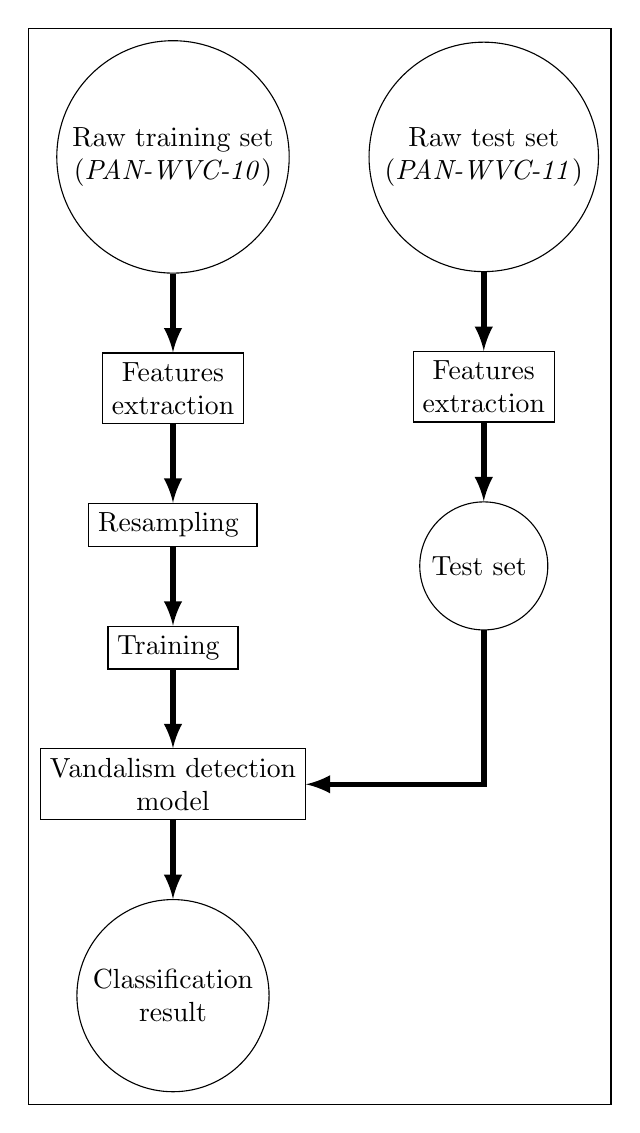
\begin{tikzpicture}[
	framed,
	nodes = {
		align = center
	},
	lines/.style={
		line width=2pt,
		>=latex
	},
	data/.style={
		circle,
		draw=black,
		text centered
	},
	proc/.style={
		rectangle,
		draw=black,
		text centered
	}
]
	\node[data] (training_raw) {
		Raw training set\\
		(\textit{PAN-WVC-10})
	};

	\node[proc] (wvcgen) [below=of training_raw] {
		Features\\
		extraction
	};

	\node[proc] (trainingset) [below=of wvcgen] {
		Resampling
	};

	\node[proc] (c)  [below=of trainingset] {
		Training
	};

	\node[proc] (m)  [below=of c] {
		Vandalism detection\\
		model
	};

	\node[data] (o)  [below=of m] {
		Classification\\
		result
	};
	%%
	\node[data] (testset_raw) [right=of training_raw] {
		Raw test set\\
		(\textit{PAN-WVC-11})
	};

	\node[proc] (testset_wvcgen) [below=of testset_raw] {
		Features\\
		extraction
	};

	\node[data] (testset) [below=of testset_wvcgen] {
		Test set
	};

	\draw[lines,->] (training_raw) -- (wvcgen);
	\draw[lines,->] (wvcgen) -- (trainingset);
	\draw[lines,->] (trainingset) -- (c);
	\draw[lines,->] (c) -- (m);
	\draw[lines,->] (m) -- (o);

	\draw[lines,->] (testset_raw) -- (testset_wvcgen);
	\draw[lines,->] (testset_wvcgen) -- (testset);

	\draw[lines,->] (testset) |- (m);
\end{tikzpicture}
}
\caption{
	Workflow process on detecting vandalism
}
\label{fig:proses}
\end{figure}


%%{{{ DATA PREPARATION
\subsection{Data Preparation}
\label{subsection:data_preparation}

The original dataset can not be used for training and testing, they need to
combined, cleaned by removing unneeded attributes, and cleaned on their content
to generate features.

Dataset that used for training is PAN-WVC-10 \cite{potthast2008automatic}.
The PAN-WVC-10 dataset contain two separate set, the edit set and
annotation set.
The edit set contain edit ID, editor (in the form of user name or IP address),
ID of old revision, ID of new revision, the URL to view the difference between
old and new revision, edit time, comment, article ID, and title of article.
The annotation set contain edit ID, class (vandalism or regular edit), number
of class annotator, and total number of annotator.

The two set then combined to get only their edit ID, class, old revision ID,
new revision ID, edit time, editor, article title, edit comment, deletions
(text that has been deleted in previous revision), and additions (text that
has been added in new revision).

The next step is to create revision text that is clean from wiki syntax, with
an aim to help in generating feature.
Every revision files cleaned up by removing URI, wiki markups, and wiki tokens.

Dataset for testing is PAN-WVC-11 \cite{potthast:2010b}.
PAN-WVC-11 contains three language set which are English, German, and Spanish.
This paper only use the English language set for testing.
The original attribute from the set is similar with PAN-WVC-10 except they were
already combined into single set, not using separate annotations.
The annotator and total annotator attributes deleted, replaced with
additions text and deletions text.
Also, the class attribute value is replaced with numeric, where
"vandalism" is become "1" and "regular" become "0".
The process for cleaning revision files is similar with PAN-WVC-10.

%%}}}

%%{{{ VANDALISM FEATURES
\subsection{Vandalism Features}

Previous papers group the features into three categories which are metadata,
text, and language.
This paper use four metadata features, 11 text features, and 10
language features which has been used and analyzed in Mola-Velasco paper
\cite{mola2012wikipedia}.

\subsubsection{Metadata Features}

Metadata feature references to the properties of revision which can be directly
taken, for example, identity of editor, comment, or the size of changes.
Below is list of metadata features,
\begin{itemize}
\item \textbf{Anonymous}. If the editor of revision is registered user then in
the edit set it contain their username. Registered user have the
value $1$, other than that will have zero value.
\item \textbf{Comment length}. Counting number of character that left by editor
in comment field without including the article's section name (usually enclosed
by \texttt{/*} and \texttt{*/}.
\item \textbf{Size increment}. An absolute size of new revision. Higher size
value can indicated as deletion on whole article.
\item \textbf{Size ratio}. The size of new revision divided by the size of old
revision.
\end{itemize}

\subsubsection{Text Features}

Below is the list of text features that are used.

\begin{itemize}
\item \textbf{Ratio of lowercase and uppercase character}. The ratio is
computed on new revision by dividing number of uppercase characters with
lowercase characters.
\item \textbf{Ratio of uppercase to all characters}. Computed by dividing
number of uppercase characters with number of all characters in new revision.
\item \textbf{Digit ratio}. Computed by dividing number of digit with number of
all character in new revision.
\item \textbf{Ratio of non-alphanumeric characters}. Computed by dividing
number of all non-alphanumeric characters with number of all characters on new
revision.
\item \textbf{Character diversity}. Computed by counting number of unique
character divided by length of text in new revision.
\item \textbf{Character distribution}. Computed using Kullback-Leibler
divergence on old revision compared with text addition in new revision.
\item \textbf{Compression rate}. Computed by applying LZW compression algorithm
on text addition divided by number of characters in additions to get their
ratio.
\item \textbf{Good token}. Computed by counting number of token that vandal
rarely used on text, for example wiki token or wiki syntax.
\item \textbf{Term frequencies}. Computed by counting number of unique words
added divided by number of unique words in new revision.
\item \textbf{Longest word}. Computed by counting number of character on the
longest word inserted.
\item \textbf{Length of similar character}. Computed by counting number of
similar characters used in sequence in single word, for example
\textit{aaarrrgghhhh}, \textit{sooo huge}.
\end{itemize}

\subsubsection{Language Features}

Language features based on number of particular words that are inserted in new
revision.
For each word categories, there are two feature to be computed: frequency and
impact.
Frequency feature computed by counting number of word in category divided by
total number of words in new revision.
Impact feature computed by counting percentage of word usage in new revision
divided by total words in old and new revision.
Below is list of language features that are used.

\begin{itemize}
\item \textbf{Vulgarism}. Counting number of vulgar, harsh, and offensive
words.
\item \textbf{Subject}. Counting number of first or second person
words used in inserted text, including colloquial words, for example
\textit{I}, \textit{you}.
\item \textbf{Bias}. Counting number of bias words, for example "coolest",
"huge".
\item \textbf{Sex}. Counting number of sex related words inserted in new
revision.
\item \textbf{Bad words}. Counting number of bad, non-vulgar, words, usually
indicated by bad writing. For example "wanna", "gotcha".
\item \textbf{All word categories}. Computed by combining all word categories
and counting each of them
\end{itemize}

%%}}}

%%{{{ GENERATING FEATURES
\subsection{Generating Feature Dataset}

All previous feature then implemented in a program.
The program than executed using PAN-WVC-10 and PAN-WVC-11 set that has been
prepared in section \ref{subsection:data_preparation}, which output dataset
feature contain continous values.
The implementation for combining, cleaning, and generating the features is
published as open source software as \texttt{wvcgen}
\footnote{\url{https://github.com/shuLhan/wvcgen}}.

%%}}}

%%{{{ RESAMPLING
\subsection{Resampling Dataset}

PAN-WVC-10 without resample contain 2,394 positive or vandalism samples and
30,045 negative or regular samples.
To get a balanced class, the dataset then resampled using SMOTE and LNSMOTE for
positive class.
For SMOTE, the parameter user for resampling is 1,100\% and parameter for
K-Nearest-Neighbour (KNN) is 5, which output 28,728 synthetic samples, total of
positive sample combined with original sample result in 31,122 positive
samples.
Parameter for resampling using LNSMOTE is similar with SMOTE, which generate
28,588 positive synthetic samples, in total of 30,892 positive samples.
The implementation for SMOTE and LNSMOTE published as open source software
\footnote{\url{https://github.com/shuLhan/go-mining/tree/master/resampling}}.

%%}}}

%%{{{ CLASSIFIER IMPLEMENTATIONS

\subsection{Classifier Implementations}

Implementation of classifiers carried out gradually.
Started by implementing CART which is used in Random Forest, which in turn is
used in Cascaded Random Forest.
The implementation of CART based on Jiawei Han et al. book, chapter 8
\cite{han2011data}.
The implementation of Random Forest is based on original paper of Breiman
\cite{breiman2001random}, plus additional resource from internet.
The implementation of Cascaded Random Forest is based on original paper of
Baumann et al.
\cite{baumann2013cascaded}.
The result of all implementation is published as open source software to help
others in future research or for real-world usage.
\footnote{\url{https://github.com/shuLhan/go-mining/tree/master/classifiers}}.

%%}}}

%%{{{ TRAINING AND TESTING
\subsection{Training and Testing}

There are three common parameter between RF and CRF which are 200 for number of
tree, 5 for number of random features, and 64\% for percentage of
bootstrapping.
For consistency, their value are constant between training.
For CRF classifier, three separated testing will be conducted using different
parameter for number of stage and number of tree which are 200 stages with 1
tree, 100 stages with 2 trees, and 50 stages with 4 trees; all of them have
equal total number of trees.
This is an experiment to see the effect of number of trees to stage and their
performance.
Another parameter for training with CRF are thresholds for true-positive rate
(TPR) and true-negative rate (TNR), which set to constant value 0.95 and 0.95
for all training.

The dataset used for training is PAN-WVC-10 which consist of three different
set, dataset without resampled, dataset resampled with SMOTE, and dataset
resampled with LNSMOTE.
The dataset used for testing is PAN-WVC-11 which contain 1,143 positive
samples and 8,842 negative samples, in total of 9985 samples.

Training is conducted by running each classifier program, RF and CRF, on
those three different PAN-WVC-10 feature dataset.
Testing is conducted after the model has been built by giving the model the
PAN-WVC-11 feature dataset as an input.

\begin{table}[tp]
\caption{Dataset for training and testing}
\label{table:dataset}
\centering
\begin{tabular}{c | l | c | c | c}
\hline
\multirow{2}{*}{Type} & \multirow{2}{*}{Resampling mode}
	& \multicolumn{3}{c}{Number of samples} \\
\cline{3-5}
    & & Vandalism & Regular & Total \\
\hline
\hline
\multirow{3}{*}{Training} & -       &  2.394 & 30.045 & 32.439 \\
                              & SMOTE   & 28.728 & 30.045 & 58.773 \\
                              & LNSMOTE & 28.588 & 30.045 & 58.633 \\
\hline
Testing & - & 1.143 & 8.842 & 9.985 \\
\hline
\end{tabular}
\end{table}


The environment used for training and testing is Intel\textregistered
Core\texttrademark i7-4750HQ CPU 2,00 GHz, with total 8 GB of RAM.
Each training is done separatedly to avoid cache miss which affect the speed
and computation time.

%%}}}

\section{Evaluation}
\label{section:result_and_analysis}

When detecting vandalism, it is better to receive false positive than missing
vandalism edit.
Wrong classification, when regular edit detected as vandalism, will give no
effect on reader, but missing on vandalism edit can lead to information loss,
fault information, or disturb the reader.
For this reason, our evaluation based on true-positive rate of classifier
performance.
True-positive rate (TPR) or recall is number of actual positive samples divided
by sum of sample positive classified as positive and sample positive classified
as negative (false-positive).
TPR has a value between 0 and 1, with value approaching to 0 indicate poor
performance and value approaching 1 indicate good performance.
Result of testing are given in terms of performance of each classifier on table
\ref{tab:stats} and training computation time on figure \ref{graph:runtimes}.

Result from CRF classifer on LNSMOTE with 200 stages and 1 tree have the
highest TPR value $0.9904$.
RF classifier without resampling gave the lowest TPR $0,1654$.

From the computation time, CRF classifier is faster than RF on all training.
Using RF and CRF with 50 stages and 4 trees as comparison, CRF without
resampling is 11 times faster than RF, and for dataset that has been resampled
with SMOTE and LNSMOTE, CRF is 1.6 times faster than RF.

\DTLsetseparator{;}
\DTLloaddb{stats}{./stats.csv}
\DTLmaxforcolumn{stats}{TPR}{\maxtpr}
\DTLminforcolumn{stats}{FPR}{\minfpr}
\DTLmaxforcolumn{stats}{TNR}{\maxtnr}
\DTLmaxforcolumn{stats}{Presisi}{\maxprec}
\DTLmaxforcolumn{stats}{F-Measure}{\maxfm}
\DTLmaxforcolumn{stats}{Akurasi}{\maxacc}
\DTLmaxforcolumn{stats}{AUC}{\maxauc}

\begin{table}[bp]
\caption{Performance of Random Forest and Cascaded Random Forest}
\centering
\begin{tabular}{llrrrrrrr}
\hline
\textbf{Classifier} &
\textbf{Dataset} &
\textbf{TPR}
\DTLforeach*{stats}{%
	\cl=Klasifikasi,%
	\ds=Dataset,%
	\tpr=TPR%
}{%
	\DTLifnullorempty{\cl}
		{\\ \cline{2-3}}
		{\\ \hline \hline}
	\DTLifnullorempty{\cl}
		{}
		{
			\multirow{3}{2cm}{\cl}
		}
	& \ds
	& \DTLifnumeq{\tpr}{\maxtpr}{\textbf{\tpr}}{\tpr}
}
\\
\hline
\end{tabular}
\label{tab:stats}
\end{table}


\begin{figure}[htbp]
\centering
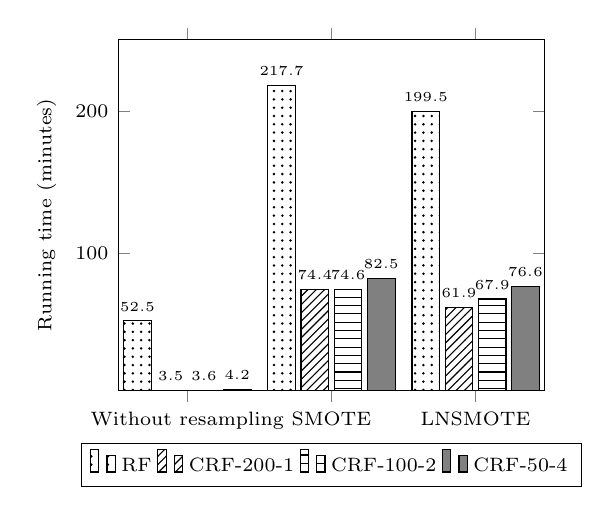
\begin{tikzpicture}[font=\scriptsize]
	\begin{axis}[
		width=7cm,
		ymax=250,
		ybar,
		ylabel=Running time (minutes),
		symbolic x coords={Without resampling, SMOTE, LNSMOTE},
		xtick=data,
		nodes near coords,
		every node near coord/.append style={font=\tiny},
		enlarge x limits=0.24,
		enlarge y limits=0,
		legend style={
			at={(0.5,-0.15)},
			anchor=north,
			legend columns=-1
		},
	]
		%% RF
		\addplot[pattern = dots] coordinates {
			(Without resampling, 52.5)
			(SMOTE, 217.7)
			(LNSMOTE, 199.5)
		};

		%% CRF-200-1
		\addplot[pattern=north east lines] coordinates {
			(Without resampling, 3.5)
			(SMOTE, 74.4)
			(LNSMOTE, 61.9)
		};

		%% CRF-100-2
		\addplot[pattern=horizontal lines] coordinates {
			(Without resampling, 3.6)
			(SMOTE, 74.6)
			(LNSMOTE, 67.9)
		};

		%% CRF-50-4
		\addplot coordinates {
			(Without resampling, 4.2)
			(SMOTE, 82.5)
			(LNSMOTE, 76.6)
		};
	\legend{RF, CRF-200-1, CRF-100-2, CRF-50-4}
	\end{axis}
\end{tikzpicture}
\caption{Running time for each classifer on different dataset.}
\label{graph:runtimes}
\end{figure}


%%{{{ Conclusion

\section{Conclusion}
\label{section:conclusion}

On average SMOTE increase TPR value by $0.19$ times while LNSMOTE, on average
increase TPR value $0.33$ times.
Another interisting effect of CRF classifier, when using less number of tree on
each stage on dataset without resampling, their performance almost similar with
CRF on resampling with more number of tree, for example performance of CRF with
100 stages and 2 tress on dataset without resampling is adjacent with CRF with
50 stages and 4 tress on dataset resampled with SMOTE.

The best classifier model for vandalism without resampling returned by CRF with
200 stages and 1 tree with TPR value $0.9668$.
The best classifier model for dataset that has been resampled with SMOTE is CRF
with 200 stage and 1 trees with TPR value $0.979$
The best classifier model for dataset that has been resampled with LNSMOTE is
CRF with 200 stages and 1 trees with TPR value $0.9904$.
Overall, the best model is CRF with 200 stages and 1 trees on dataset resampled
with LNSMOTE.
Beside their good performance result, CRF on average $1.6$ times faster at
training than RF on resampled dataset.

\section{Contribution}

This paper contribute on finding the best classifier on detecting vandalism on
Wikipedia and evaluating the effect of LNSMOTE resampling on imbalance dataset
and performance of CRF agains RF.
Apart from that, this paper also provide a framework to create and develop
vandalism features from raw PAN WVC dataset without having to build it again
from scratch.
Another contribution is a library for data processing and machine learning,
especially on resampling using LNSMOTE and CRF classifier which has no
open implementation on renowed program like Weka, Scikit-Learn, or R.
This framework can be used in the next research or in real-world application.

\section{Future Works}

The number of internet users and Indonesian articles in Wikipedia is keep
growing each years.
The more users then the more prone the wiki to vandalism.
Before an editor can catch up with number of users, it would be better if
Indonesian Wikipedia have a better system to detect vandalism.
Collecting an annotated vandalism articles on Wikipedia Indonesia could be
good start before learning or creating the system to counter it.

All of training model on this paper still using RF and CRF algorithm in serial,
in which each tree is build one by one sequentially or when classifying sample,
each of them was given as input to each tree sequentially to get their class.
Using parallel algorithm, for trees building or classifying samples, can
speeding up training, testing and getting classifier result.
On domain of machine learning, an interesting new algorithm is eXtreme
Gradient Boostring (XGBoost)
\cite{chen2016xgboost}.
Using XGBoost on Wikipedia vandalism dataset maybe can increase the accuracy
of detection.

%%}}}

\IEEEtriggeratref{10}
\bibliographystyle{IEEEtran}
\bibliography{IEEEabrv,bibliography}

\end{document}
